\documentclass{standalone}
\usepackage{tikz}
\usetikzlibrary{patterns, positioning}


\begin{document}
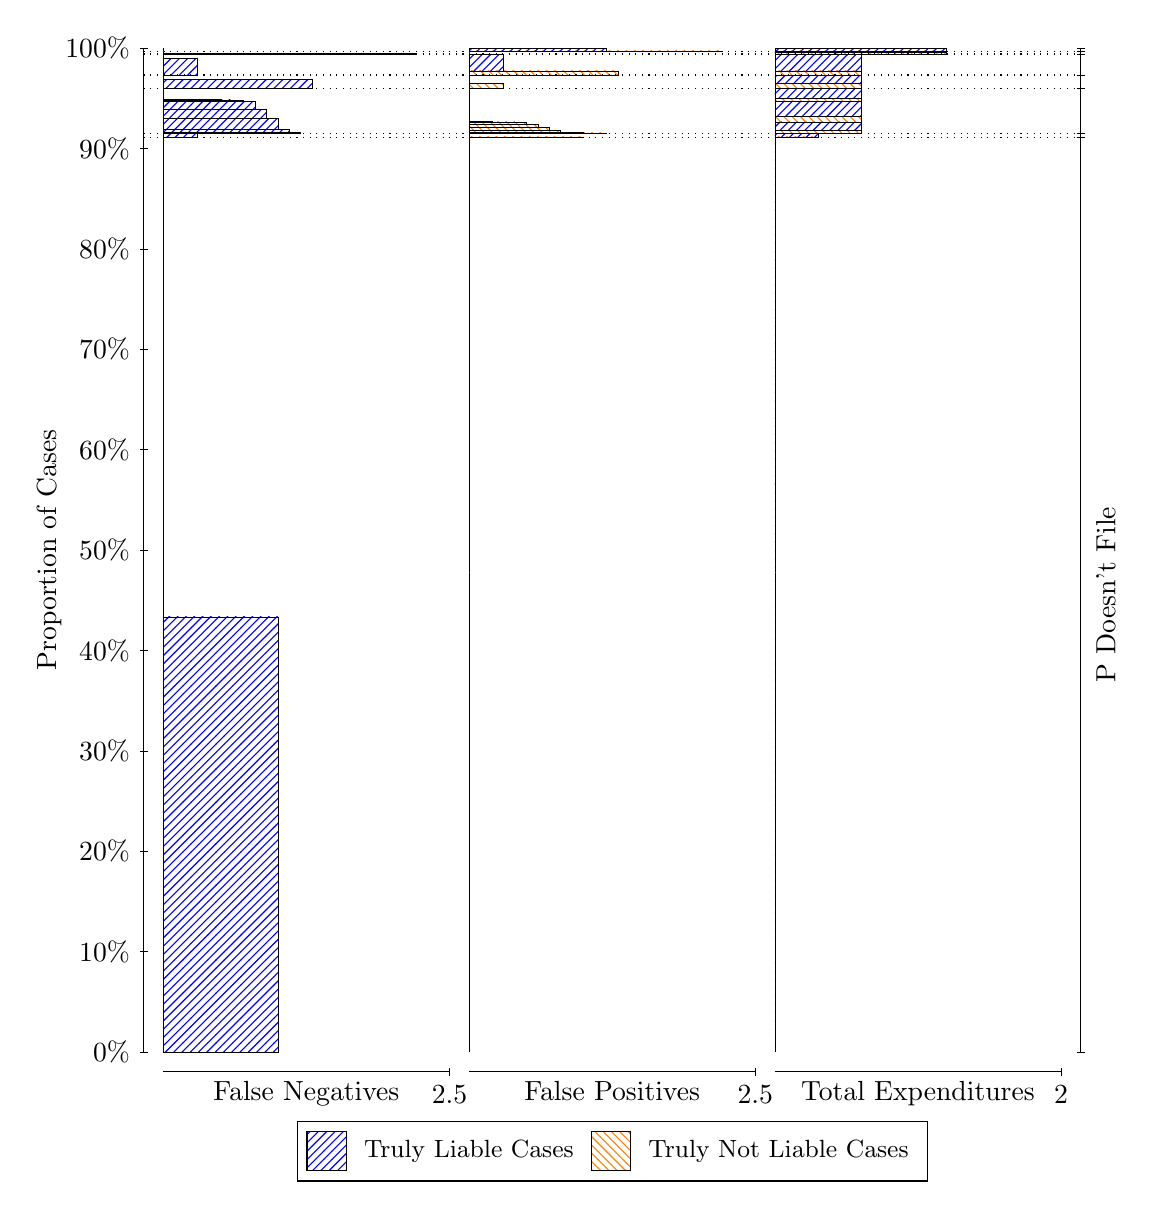
\begin{tikzpicture}
\draw[black, very thin] (1.5,1.75) -- (1.5,14.5);
\node[rotate=90, text=black, anchor=center] at (0.3, 8.125) {Proportion of Cases};
\draw[black, very thin] (1.45,1.75) -- (1.55,1.75);
\node[text=black, anchor=east] at (1.45, 1.75) {0\%};
\draw[black, very thin] (1.45,3.025) -- (1.55,3.025);
\node[text=black, anchor=east] at (1.45, 3.025) {10\%};
\draw[black, very thin] (1.45,4.3) -- (1.55,4.3);
\node[text=black, anchor=east] at (1.45, 4.3) {20\%};
\draw[black, very thin] (1.45,5.575) -- (1.55,5.575);
\node[text=black, anchor=east] at (1.45, 5.575) {30\%};
\draw[black, very thin] (1.45,6.85) -- (1.55,6.85);
\node[text=black, anchor=east] at (1.45, 6.85) {40\%};
\draw[black, very thin] (1.45,8.125) -- (1.55,8.125);
\node[text=black, anchor=east] at (1.45, 8.125) {50\%};
\draw[black, very thin] (1.45,9.4) -- (1.55,9.4);
\node[text=black, anchor=east] at (1.45, 9.4) {60\%};
\draw[black, very thin] (1.45,10.675) -- (1.55,10.675);
\node[text=black, anchor=east] at (1.45, 10.675) {70\%};
\draw[black, very thin] (1.45,11.95) -- (1.55,11.95);
\node[text=black, anchor=east] at (1.45, 11.95) {80\%};
\draw[black, very thin] (1.45,13.225) -- (1.55,13.225);
\node[text=black, anchor=east] at (1.45, 13.225) {90\%};
\draw[black, very thin] (1.45,14.5) -- (1.55,14.5);
\node[text=black, anchor=east] at (1.45, 14.5) {100\%};

\draw[black, very thin] (13.4,1.75) -- (13.4,14.5);
\draw[black, very thin] (13.35,1.75) -- (13.45,1.75);
\node[anchor=west] at (13.35, 1.75) {};
\draw[black, very thin] (13.35,13.367) -- (13.45,13.367);
\node[anchor=west] at (13.35, 13.367) {};
\draw[black, very thin] (13.35,13.42) -- (13.45,13.42);
\node[anchor=west] at (13.35, 13.42) {};
\draw[black, very thin] (13.35,13.99) -- (13.45,13.99);
\node[anchor=west] at (13.35, 13.99) {};
\draw[black, very thin] (13.35,14.157) -- (13.45,14.157);
\node[anchor=west] at (13.35, 14.157) {};
\draw[black, very thin] (13.35,14.424) -- (13.45,14.424);
\node[anchor=west] at (13.35, 14.424) {};
\draw[black, very thin] (13.35,14.455) -- (13.45,14.455);
\node[anchor=west] at (13.35, 14.455) {};
\draw[black, very thin] (13.35,14.5) -- (13.45,14.5);
\node[anchor=west] at (13.35, 14.5) {};

\draw[black, very thin, pattern color=blue, pattern=north east lines] (1.75,1.75) rectangle (3.2033,7.2769);
\draw[black, very thin, pattern color=orange, pattern=north west lines] (1.75,7.2769) rectangle (1.75,13.367);
\draw[black, very thin, pattern color=blue, pattern=north east lines] (1.75,13.367) rectangle (2.186,13.415);
\draw[black, very thin, pattern color=orange, pattern=north west lines] (1.75,13.415) rectangle (1.75,13.42);
\draw[black, very thin, pattern color=blue, pattern=north east lines] (1.75,13.42) rectangle (3.494,13.432);
\draw[black, very thin, pattern color=blue, pattern=north east lines] (1.75,13.432) rectangle (3.3487,13.467);
\draw[black, very thin, pattern color=blue, pattern=north east lines] (1.75,13.467) rectangle (3.2033,13.603);
\draw[black, very thin, pattern color=blue, pattern=north east lines] (1.75,13.603) rectangle (3.058,13.607);
\draw[black, very thin, pattern color=blue, pattern=north east lines] (1.75,13.607) rectangle (3.058,13.724);
\draw[black, very thin, pattern color=blue, pattern=north east lines] (1.75,13.724) rectangle (2.9127,13.825);
\draw[black, very thin, pattern color=blue, pattern=north east lines] (1.75,13.825) rectangle (2.7673,13.833);
\draw[black, very thin, pattern color=blue, pattern=north east lines] (1.75,13.833) rectangle (2.622,13.841);
\draw[black, very thin, pattern color=blue, pattern=north east lines] (1.75,13.841) rectangle (2.4767,13.845);
\draw[black, very thin, pattern color=blue, pattern=north east lines] (1.75,13.845) rectangle (2.3313,13.849);
\draw[black, very thin, pattern color=orange, pattern=north west lines] (1.75,13.849) rectangle (1.75,13.99);
\draw[black, very thin, pattern color=blue, pattern=north east lines] (1.75,13.99) rectangle (3.6393,14.101);
\draw[black, very thin, pattern color=orange, pattern=north west lines] (1.75,14.101) rectangle (1.75,14.157);
\draw[black, very thin, pattern color=blue, pattern=north east lines] (1.75,14.157) rectangle (2.186,14.372);
\draw[black, very thin, pattern color=orange, pattern=north west lines] (1.75,14.372) rectangle (1.75,14.424);
\draw[black, very thin, pattern color=blue, pattern=north east lines] (1.75,14.424) rectangle (4.9473,14.433);
\draw[black, very thin, pattern color=orange, pattern=north west lines] (1.75,14.433) rectangle (1.75,14.455);
\draw[black, very thin, pattern color=orange, pattern=north west lines] (1.75,14.455) rectangle (1.75,14.464);
\draw[black, very thin, pattern color=blue, pattern=north east lines] (1.75,14.464) rectangle (1.75,14.5);
\draw[black, very thin, pattern color=orange, pattern=north west lines] (5.6333,1.75) rectangle (5.6333,7.8405);
\draw[black, very thin, pattern color=blue, pattern=north east lines] (5.6333,7.8405) rectangle (5.6333,13.367);
\draw[black, very thin, pattern color=orange, pattern=north west lines] (5.6333,13.367) rectangle (7.0867,13.372);
\draw[black, very thin, pattern color=blue, pattern=north east lines] (5.6333,13.372) rectangle (5.6333,13.42);
\draw[black, very thin, pattern color=orange, pattern=north west lines] (5.6333,13.42) rectangle (7.3773,13.421);
\draw[black, very thin, pattern color=orange, pattern=north west lines] (5.6333,13.421) rectangle (7.232,13.423);
\draw[black, very thin, pattern color=orange, pattern=north west lines] (5.6333,13.423) rectangle (7.0867,13.426);
\draw[black, very thin, pattern color=orange, pattern=north west lines] (5.6333,13.426) rectangle (6.9413,13.429);
\draw[black, very thin, pattern color=orange, pattern=north west lines] (5.6333,13.429) rectangle (6.796,13.456);
\draw[black, very thin, pattern color=orange, pattern=north west lines] (5.6333,13.456) rectangle (6.6507,13.489);
\draw[black, very thin, pattern color=orange, pattern=north west lines] (5.6333,13.489) rectangle (6.5053,13.535);
\draw[black, very thin, pattern color=orange, pattern=north west lines] (5.6333,13.535) rectangle (6.36,13.552);
\draw[black, very thin, pattern color=orange, pattern=north west lines] (5.6333,13.552) rectangle (6.2147,13.561);
\draw[black, very thin, pattern color=blue, pattern=north east lines] (5.6333,13.561) rectangle (5.924,13.565);
\draw[black, very thin, pattern color=blue, pattern=north east lines] (5.6333,13.565) rectangle (5.7787,13.569);
\draw[black, very thin, pattern color=blue, pattern=north east lines] (5.6333,13.569) rectangle (5.6333,13.99);
\draw[black, very thin, pattern color=orange, pattern=north west lines] (5.6333,13.99) rectangle (6.0693,14.046);
\draw[black, very thin, pattern color=blue, pattern=north east lines] (5.6333,14.046) rectangle (5.6333,14.157);
\draw[black, very thin, pattern color=orange, pattern=north west lines] (5.6333,14.157) rectangle (7.5227,14.209);
\draw[black, very thin, pattern color=blue, pattern=north east lines] (5.6333,14.209) rectangle (6.0693,14.424);
\draw[black, very thin, pattern color=orange, pattern=north west lines] (5.6333,14.424) rectangle (5.6333,14.445);
\draw[black, very thin, pattern color=blue, pattern=north east lines] (5.6333,14.445) rectangle (5.6333,14.455);
\draw[black, very thin, pattern color=orange, pattern=north west lines] (5.6333,14.455) rectangle (8.8307,14.464);
\draw[black, very thin, pattern color=blue, pattern=north east lines] (5.6333,14.464) rectangle (7.3773,14.5);
\draw[black, very thin, pattern color=orange, pattern=north west lines] (9.5167,1.75) rectangle (9.5167,7.8405);
\draw[black, very thin, pattern color=blue, pattern=north east lines] (9.5167,7.8405) rectangle (9.5167,13.367);
\draw[black, very thin, pattern color=orange, pattern=north west lines] (9.5167,13.367) rectangle (10.062,13.372);
\draw[black, very thin, pattern color=blue, pattern=north east lines] (9.5167,13.372) rectangle (10.062,13.42);
\draw[black, very thin, pattern color=orange, pattern=north west lines] (9.5167,13.42) rectangle (10.607,13.451);
\draw[black, very thin, pattern color=blue, pattern=north east lines] (9.5167,13.451) rectangle (10.607,13.563);
\draw[black, very thin, pattern color=orange, pattern=north west lines] (9.5167,13.563) rectangle (10.607,13.636);
\draw[black, very thin, pattern color=blue, pattern=north east lines] (9.5167,13.636) rectangle (10.607,13.823);
\draw[black, very thin, pattern color=orange, pattern=north west lines] (9.5167,13.823) rectangle (10.607,13.86);
\draw[black, very thin, pattern color=blue, pattern=north east lines] (9.5167,13.86) rectangle (10.607,13.99);
\draw[black, very thin, pattern color=orange, pattern=north west lines] (9.5167,13.99) rectangle (10.607,14.046);
\draw[black, very thin, pattern color=blue, pattern=north east lines] (9.5167,14.046) rectangle (10.607,14.157);
\draw[black, very thin, pattern color=orange, pattern=north west lines] (9.5167,14.157) rectangle (10.607,14.209);
\draw[black, very thin, pattern color=blue, pattern=north east lines] (9.5167,14.209) rectangle (10.607,14.424);
\draw[black, very thin, pattern color=orange, pattern=north west lines] (9.5167,14.424) rectangle (11.697,14.445);
\draw[black, very thin, pattern color=blue, pattern=north east lines] (9.5167,14.445) rectangle (11.697,14.455);
\draw[black, very thin, pattern color=orange, pattern=north west lines] (9.5167,14.455) rectangle (11.697,14.464);
\draw[black, very thin, pattern color=blue, pattern=north east lines] (9.5167,14.464) rectangle (11.697,14.5);
\draw[black, dotted] (1.5,13.367) -- (13.4,13.367);
\draw[black, dotted] (1.5,13.42) -- (13.4,13.42);
\draw[black, dotted] (1.5,13.99) -- (13.4,13.99);
\draw[black, dotted] (1.5,14.157) -- (13.4,14.157);
\draw[black, dotted] (1.5,14.424) -- (13.4,14.424);
\draw[black, dotted] (1.5,14.455) -- (13.4,14.455);
\draw[black, very thin] (1.75,1.5) -- (5.3833,1.5);
\node[text=black, anchor=north] at (3.5667, 1.5) {False Negatives};
\draw[black, very thin] (5.3833,1.45) -- (5.3833,1.55);
\node[text=black, anchor=north] at (5.3833, 1.45) {2.5};

\draw[black, very thin] (5.6333,1.5) -- (9.2667,1.5);
\node[text=black, anchor=north] at (7.45, 1.5) {False Positives};
\draw[black, very thin] (9.2667,1.45) -- (9.2667,1.55);
\node[text=black, anchor=north] at (9.2667, 1.45) {2.5};

\draw[black, very thin] (9.5167,1.5) -- (13.15,1.5);
\node[text=black, anchor=north] at (11.333, 1.5) {Total Expenditures};
\draw[black, very thin] (13.15,1.45) -- (13.15,1.55);
\node[text=black, anchor=north] at (13.15, 1.45) {2};

\node[text=black, centered, rotate=90] at (13.72, 7.5587) {P Doesn't File};







\draw (7.449999999999999,1.5) node[draw=none] (baseCoordinate) {};
\begin{scope}[align=center]
        \matrix[scale=0.5, draw=black, below=0.5cm of baseCoordinate, nodes={draw}, column sep=0.1cm]{
            \node[rectangle, draw, minimum width=0.5cm, minimum height=0.5cm, pattern color=blue, pattern=north east lines] {}; &
            \node[draw=none, font=\small, text=black] (B) {Truly Liable Cases}; &
            \node[rectangle, draw, minimum width=0.5cm, minimum height=0.5cm, pattern color=orange, pattern=north west lines] {}; &
            \node[draw=none, font=\small, text=black] (B) {Truly Not Liable Cases}; \\
            };
\end{scope}

\end{tikzpicture}
\end{document}